\begin{figure*}[ht]
\begin{center}
\begin{adjustbox}{width=0.7\textwidth}

    \tikzset{every picture/.style={line width=0.75pt}} %set default line width to 0.75pt        
    
    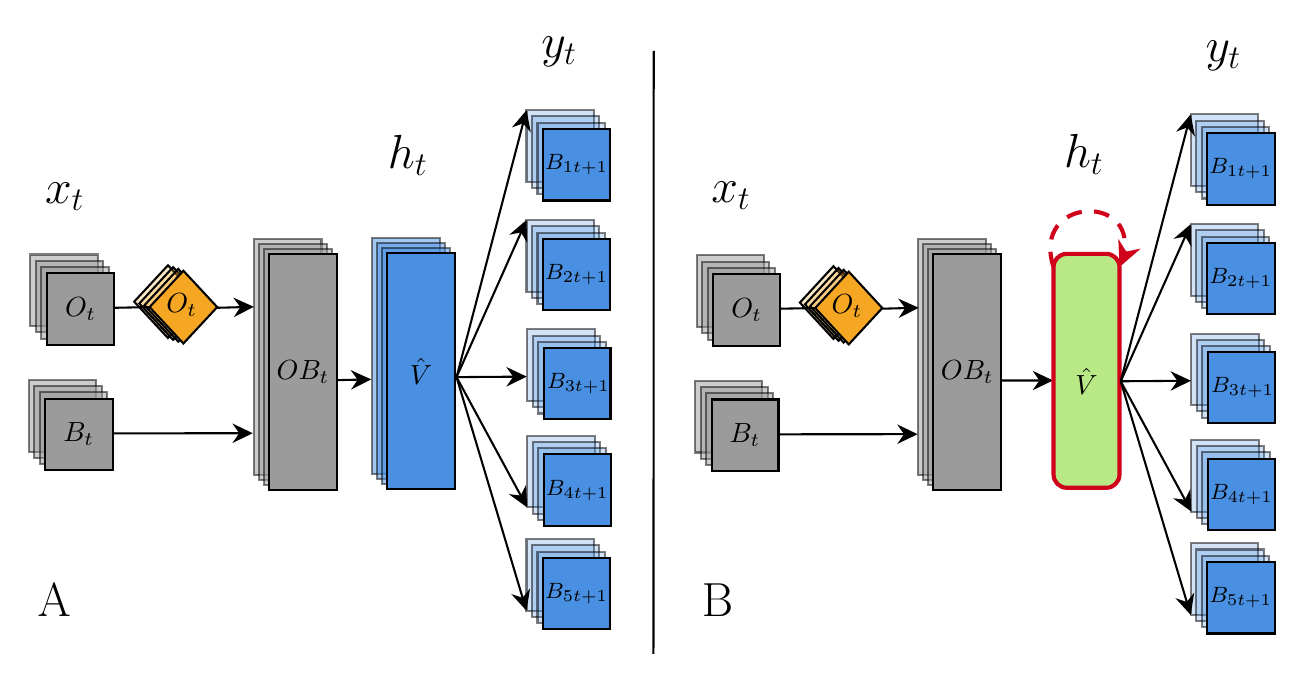
\begin{tikzpicture}[x=0.75pt,y=0.75pt,yscale=-1,xscale=1]
    %uncomment if require: \path (0,359); %set diagram left start at 0, and has height of 359
    
    %Shape: Diamond [id:dp8512741780313259] 
    \draw  [fill={rgb, 255:red, 245; green, 166; blue, 35 }  ,fill opacity=0.25 ] (76.97,133.57) -- (93.27,151.09) -- (76.97,168.6) -- (60.68,151.09) -- cycle ;
    %Shape: Diamond [id:dp44131568061643844] 
    \draw  [fill={rgb, 255:red, 245; green, 166; blue, 35 }  ,fill opacity=0.25 ] (79.45,134.45) -- (95.74,151.96) -- (79.45,169.48) -- (63.15,151.96) -- cycle ;
    %Shape: Diamond [id:dp9944377463655836] 
    \draw  [fill={rgb, 255:red, 245; green, 166; blue, 35 }  ,fill opacity=0.25 ] (81.92,135.32) -- (98.22,152.84) -- (81.92,170.35) -- (65.63,152.84) -- cycle ;
    %Shape: Rectangle [id:dp3605470636117536] 
    \draw  [color={rgb, 255:red, 0; green, 0; blue, 0 }  ,draw opacity=0.5 ][fill={rgb, 255:red, 74; green, 144; blue, 226 }  ,fill opacity=0.5 ] (175.1,120.3) -- (207.87,120.3) -- (207.87,234) -- (175.1,234) -- cycle ;
    %Shape: Rectangle [id:dp7194333726509892] 
    \draw  [color={rgb, 255:red, 0; green, 0; blue, 0 }  ,draw opacity=0.5 ][fill={rgb, 255:red, 74; green, 144; blue, 226 }  ,fill opacity=0.5 ] (177.57,122.76) -- (210.34,122.76) -- (210.34,236.46) -- (177.57,236.46) -- cycle ;
    %Shape: Rectangle [id:dp3276084138933598] 
    \draw  [color={rgb, 255:red, 0; green, 0; blue, 0 }  ,draw opacity=0.5 ][fill={rgb, 255:red, 74; green, 144; blue, 226 }  ,fill opacity=0.5 ] (180.05,125.22) -- (212.82,125.22) -- (212.82,238.92) -- (180.05,238.92) -- cycle ;
    %Shape: Diamond [id:dp6965315978812838] 
    \draw  [fill={rgb, 255:red, 245; green, 166; blue, 35 }  ,fill opacity=1 ] (84.4,136.2) -- (100.69,153.71) -- (84.4,171.23) -- (68.1,153.71) -- cycle ;
    %Straight Lines [id:da5408632178702979] 
    \draw    (100.5,154.05) -- (115.35,153.66) ;
    \draw [shift={(118.35,153.58)}, rotate = 538.5] [fill={rgb, 255:red, 0; green, 0; blue, 0 }  ][line width=0.08]  [draw opacity=0] (9.82,-4.72) -- (0,0) -- (9.82,4.72) -- (6.52,0) -- cycle    ;
    %Straight Lines [id:da38550305545794683] 
    \draw [fill={rgb, 255:red, 155; green, 155; blue, 155 }  ,fill opacity=1 ]   (28.09,214.56) -- (114.82,214.48) ;
    \draw [shift={(117.82,214.48)}, rotate = 539.95] [fill={rgb, 255:red, 0; green, 0; blue, 0 }  ][line width=0.08]  [draw opacity=0] (9.82,-4.72) -- (0,0) -- (9.82,4.72) -- (6.52,0) -- cycle    ;
    %Shape: Rectangle [id:dp8586026364143547] 
    \draw  [color={rgb, 255:red, 0; green, 0; blue, 0 }  ,draw opacity=0.5 ][fill={rgb, 255:red, 74; green, 144; blue, 226 }  ,fill opacity=0.25 ] (249.7,111.78) -- (282.2,111.78) -- (282.2,146.29) -- (249.7,146.29) -- cycle ;
    %Shape: Rectangle [id:dp5271658440371366] 
    \draw  [color={rgb, 255:red, 0; green, 0; blue, 0 }  ,draw opacity=0.5 ][fill={rgb, 255:red, 74; green, 144; blue, 226 }  ,fill opacity=0.25 ] (252.34,114.76) -- (284.84,114.76) -- (284.84,149.27) -- (252.34,149.27) -- cycle ;
    %Shape: Rectangle [id:dp6121896210605144] 
    \draw  [color={rgb, 255:red, 0; green, 0; blue, 0 }  ,draw opacity=0.5 ][fill={rgb, 255:red, 74; green, 144; blue, 226 }  ,fill opacity=0.25 ] (255,117.81) -- (287.51,117.81) -- (287.51,152.32) -- (255,152.32) -- cycle ;
    %Shape: Rectangle [id:dp2571940122217342] 
    \draw  [fill={rgb, 255:red, 74; green, 144; blue, 226 }  ,fill opacity=1 ] (257.61,120.75) -- (290.11,120.75) -- (290.11,155.25) -- (257.61,155.25) -- cycle ;
    %Shape: Rectangle [id:dp04921858860159267] 
    \draw  [color={rgb, 255:red, 0; green, 0; blue, 0 }  ,draw opacity=0.5 ][fill={rgb, 255:red, 74; green, 144; blue, 226 }  ,fill opacity=0.25 ] (250.03,164.45) -- (282.53,164.45) -- (282.53,198.95) -- (250.03,198.95) -- cycle ;
    %Shape: Rectangle [id:dp5512084563866699] 
    \draw  [color={rgb, 255:red, 0; green, 0; blue, 0 }  ,draw opacity=0.5 ][fill={rgb, 255:red, 74; green, 144; blue, 226 }  ,fill opacity=0.25 ] (252.67,167.43) -- (285.17,167.43) -- (285.17,201.93) -- (252.67,201.93) -- cycle ;
    %Shape: Rectangle [id:dp948946889597384] 
    \draw  [color={rgb, 255:red, 0; green, 0; blue, 0 }  ,draw opacity=0.5 ][fill={rgb, 255:red, 74; green, 144; blue, 226 }  ,fill opacity=0.25 ] (255.33,170.48) -- (287.84,170.48) -- (287.84,204.98) -- (255.33,204.98) -- cycle ;
    %Shape: Rectangle [id:dp7446725750615967] 
    \draw  [fill={rgb, 255:red, 74; green, 144; blue, 226 }  ,fill opacity=1 ] (257.95,173.41) -- (290.17,173.41) -- (290.17,207.61) -- (257.95,207.61) -- cycle ;
    %Shape: Rectangle [id:dp2953756097578333] 
    \draw  [color={rgb, 255:red, 0; green, 0; blue, 0 }  ,draw opacity=0.5 ][fill={rgb, 255:red, 74; green, 144; blue, 226 }  ,fill opacity=0.25 ] (249.7,265.5) -- (282.2,265.5) -- (282.2,300.01) -- (249.7,300.01) -- cycle ;
    %Shape: Rectangle [id:dp8190984811103563] 
    \draw  [color={rgb, 255:red, 0; green, 0; blue, 0 }  ,draw opacity=0.5 ][fill={rgb, 255:red, 74; green, 144; blue, 226 }  ,fill opacity=0.25 ] (252.34,268.48) -- (284.84,268.48) -- (284.84,302.99) -- (252.34,302.99) -- cycle ;
    %Shape: Rectangle [id:dp1989563986467071] 
    \draw  [color={rgb, 255:red, 0; green, 0; blue, 0 }  ,draw opacity=0.5 ][fill={rgb, 255:red, 74; green, 144; blue, 226 }  ,fill opacity=0.25 ] (255,271.53) -- (287.51,271.53) -- (287.51,306.04) -- (255,306.04) -- cycle ;
    %Shape: Rectangle [id:dp1924397511107222] 
    \draw  [fill={rgb, 255:red, 74; green, 144; blue, 226 }  ,fill opacity=1 ] (257.61,274.47) -- (290.11,274.47) -- (290.11,308.98) -- (257.61,308.98) -- cycle ;
    %Shape: Rectangle [id:dp8187051960536611] 
    \draw  [color={rgb, 255:red, 0; green, 0; blue, 0 }  ,draw opacity=0.5 ][fill={rgb, 255:red, 74; green, 144; blue, 226 }  ,fill opacity=0.25 ] (250.03,215.71) -- (282.53,215.71) -- (282.53,250.22) -- (250.03,250.22) -- cycle ;
    %Shape: Rectangle [id:dp6023578581008111] 
    \draw  [color={rgb, 255:red, 0; green, 0; blue, 0 }  ,draw opacity=0.5 ][fill={rgb, 255:red, 74; green, 144; blue, 226 }  ,fill opacity=0.25 ] (252.67,218.69) -- (285.17,218.69) -- (285.17,253.2) -- (252.67,253.2) -- cycle ;
    %Shape: Rectangle [id:dp8798703561171738] 
    \draw  [color={rgb, 255:red, 0; green, 0; blue, 0 }  ,draw opacity=0.5 ][fill={rgb, 255:red, 74; green, 144; blue, 226 }  ,fill opacity=0.25 ] (255.33,221.74) -- (287.84,221.74) -- (287.84,256.25) -- (255.33,256.25) -- cycle ;
    %Shape: Rectangle [id:dp3283044450373016] 
    \draw  [fill={rgb, 255:red, 74; green, 144; blue, 226 }  ,fill opacity=1 ] (257.94,224.68) -- (290.44,224.68) -- (290.44,259.19) -- (257.94,259.19) -- cycle ;
    %Shape: Rectangle [id:dp15154204076473643] 
    \draw  [color={rgb, 255:red, 0; green, 0; blue, 0 }  ,draw opacity=0.5 ][fill={rgb, 255:red, 155; green, 155; blue, 155 }  ,fill opacity=0.5 ] (9.87,188.8) -- (42.37,188.8) -- (42.37,223.31) -- (9.87,223.31) -- cycle ;
    %Shape: Rectangle [id:dp9182207029607203] 
    \draw  [color={rgb, 255:red, 0; green, 0; blue, 0 }  ,draw opacity=0.5 ][fill={rgb, 255:red, 155; green, 155; blue, 155 }  ,fill opacity=0.5 ] (12.51,191.78) -- (45.01,191.78) -- (45.01,226.28) -- (12.51,226.28) -- cycle ;
    %Shape: Rectangle [id:dp7698171692832448] 
    \draw  [color={rgb, 255:red, 0; green, 0; blue, 0 }  ,draw opacity=0.5 ][fill={rgb, 255:red, 155; green, 155; blue, 155 }  ,fill opacity=0.5 ] (15.17,194.83) -- (47.68,194.83) -- (47.68,229.34) -- (15.17,229.34) -- cycle ;
    %Shape: Rectangle [id:dp3865383455450443] 
    \draw  [fill={rgb, 255:red, 155; green, 155; blue, 155 }  ,fill opacity=1 ] (17.78,197.77) -- (50.28,197.77) -- (50.28,232.27) -- (17.78,232.27) -- cycle ;
    %Shape: Rectangle [id:dp23172130161456372] 
    \draw  [fill={rgb, 255:red, 74; green, 144; blue, 226 }  ,fill opacity=1 ] (182.52,127.67) -- (215.29,127.67) -- (215.29,241.37) -- (182.52,241.37) -- cycle ;
    %Shape: Rectangle [id:dp18125329077839125] 
    \draw  [color={rgb, 255:red, 0; green, 0; blue, 0 }  ,draw opacity=0.5 ][fill={rgb, 255:red, 74; green, 144; blue, 226 }  ,fill opacity=0.25 ] (249.7,58.87) -- (282.2,58.87) -- (282.2,93.37) -- (249.7,93.37) -- cycle ;
    %Shape: Rectangle [id:dp3729389269249752] 
    \draw  [color={rgb, 255:red, 0; green, 0; blue, 0 }  ,draw opacity=0.5 ][fill={rgb, 255:red, 74; green, 144; blue, 226 }  ,fill opacity=0.25 ] (252.34,61.84) -- (284.84,61.84) -- (284.84,96.35) -- (252.34,96.35) -- cycle ;
    %Shape: Rectangle [id:dp8889532693849542] 
    \draw  [color={rgb, 255:red, 0; green, 0; blue, 0 }  ,draw opacity=0.5 ][fill={rgb, 255:red, 74; green, 144; blue, 226 }  ,fill opacity=0.25 ] (255,64.9) -- (287.51,64.9) -- (287.51,99.4) -- (255,99.4) -- cycle ;
    %Shape: Rectangle [id:dp22768677359456946] 
    \draw  [fill={rgb, 255:red, 74; green, 144; blue, 226 }  ,fill opacity=1 ] (257.61,67.83) -- (290.11,67.83) -- (290.11,102.34) -- (257.61,102.34) -- cycle ;
    %Straight Lines [id:da6521632540749734] 
    \draw    (216,187.45) -- (248.94,61.77) ;
    \draw [shift={(249.7,58.87)}, rotate = 464.68] [fill={rgb, 255:red, 0; green, 0; blue, 0 }  ][line width=0.08]  [draw opacity=0] (9.82,-4.72) -- (0,0) -- (9.82,4.72) -- (6.52,0) -- cycle    ;
    %Straight Lines [id:da4098284445759105] 
    \draw    (216,187.45) -- (248.48,114.52) ;
    \draw [shift={(249.7,111.78)}, rotate = 474] [fill={rgb, 255:red, 0; green, 0; blue, 0 }  ][line width=0.08]  [draw opacity=0] (9.82,-4.72) -- (0,0) -- (9.82,4.72) -- (6.52,0) -- cycle    ;
    %Straight Lines [id:da6632019398295455] 
    \draw    (216,187.45) -- (246.8,187.22) ;
    \draw [shift={(249.8,187.2)}, rotate = 539.5699999999999] [fill={rgb, 255:red, 0; green, 0; blue, 0 }  ][line width=0.08]  [draw opacity=0] (9.82,-4.72) -- (0,0) -- (9.82,4.72) -- (6.52,0) -- cycle    ;
    %Straight Lines [id:da3742350341861914] 
    \draw    (216,187.45) -- (248.6,247.58) ;
    \draw [shift={(250.03,250.22)}, rotate = 241.54] [fill={rgb, 255:red, 0; green, 0; blue, 0 }  ][line width=0.08]  [draw opacity=0] (9.82,-4.72) -- (0,0) -- (9.82,4.72) -- (6.52,0) -- cycle    ;
    %Straight Lines [id:da8736791937763184] 
    \draw    (216,187.45) -- (248.84,297.14) ;
    \draw [shift={(249.7,300.01)}, rotate = 253.32999999999998] [fill={rgb, 255:red, 0; green, 0; blue, 0 }  ][line width=0.08]  [draw opacity=0] (9.82,-4.72) -- (0,0) -- (9.82,4.72) -- (6.52,0) -- cycle    ;
    %Shape: Rectangle [id:dp20286680685222525] 
    \draw  [color={rgb, 255:red, 0; green, 0; blue, 0 }  ,draw opacity=0.5 ][fill={rgb, 255:red, 155; green, 155; blue, 155 }  ,fill opacity=0.5 ] (10.69,128.37) -- (43.2,128.37) -- (43.2,162.88) -- (10.69,162.88) -- cycle ;
    %Shape: Rectangle [id:dp3612691236911778] 
    \draw  [color={rgb, 255:red, 0; green, 0; blue, 0 }  ,draw opacity=0.5 ][fill={rgb, 255:red, 155; green, 155; blue, 155 }  ,fill opacity=0.5 ] (13.33,131.35) -- (45.84,131.35) -- (45.84,165.85) -- (13.33,165.85) -- cycle ;
    %Shape: Rectangle [id:dp27994822217022974] 
    \draw  [color={rgb, 255:red, 0; green, 0; blue, 0 }  ,draw opacity=0.5 ][fill={rgb, 255:red, 155; green, 155; blue, 155 }  ,fill opacity=0.5 ] (16,134.4) -- (48.5,134.4) -- (48.5,168.91) -- (16,168.91) -- cycle ;
    %Shape: Rectangle [id:dp8551279256791401] 
    \draw  [fill={rgb, 255:red, 155; green, 155; blue, 155 }  ,fill opacity=1 ] (18.6,137.34) -- (51.11,137.34) -- (51.11,171.84) -- (18.6,171.84) -- cycle ;
    %Straight Lines [id:da9406188534668796] 
    \draw    (51,154.05) -- (68.1,153.71) ;
    %Shape: Diamond [id:dp9716226680975282] 
    \draw  [fill={rgb, 255:red, 245; green, 166; blue, 35 }  ,fill opacity=0.25 ] (397.6,134.01) -- (413.77,151.53) -- (397.6,169.05) -- (381.43,151.53) -- cycle ;
    %Shape: Diamond [id:dp8853919017185783] 
    \draw  [fill={rgb, 255:red, 245; green, 166; blue, 35 }  ,fill opacity=0.25 ] (400.05,134.88) -- (416.22,152.4) -- (400.05,169.93) -- (383.89,152.4) -- cycle ;
    %Shape: Diamond [id:dp4795794552356232] 
    \draw  [fill={rgb, 255:red, 245; green, 166; blue, 35 }  ,fill opacity=0.25 ] (402.51,135.76) -- (418.68,153.28) -- (402.51,170.8) -- (386.34,153.28) -- cycle ;
    %Shape: Rectangle [id:dp9874370088724661] 
    \draw  [color={rgb, 255:red, 0; green, 0; blue, 0 }  ,draw opacity=0.5 ][fill={rgb, 255:red, 155; green, 155; blue, 155 }  ,fill opacity=0.5 ] (438.41,120.73) -- (470.92,120.73) -- (470.92,234.47) -- (438.41,234.47) -- cycle ;
    %Shape: Rectangle [id:dp4226010417229218] 
    \draw  [color={rgb, 255:red, 0; green, 0; blue, 0 }  ,draw opacity=0.5 ][fill={rgb, 255:red, 155; green, 155; blue, 155 }  ,fill opacity=0.5 ] (440.86,123.19) -- (473.38,123.19) -- (473.38,236.93) -- (440.86,236.93) -- cycle ;
    %Shape: Rectangle [id:dp4167988625262439] 
    \draw  [color={rgb, 255:red, 0; green, 0; blue, 0 }  ,draw opacity=0.5 ][fill={rgb, 255:red, 155; green, 155; blue, 155 }  ,fill opacity=0.5 ] (443.32,125.65) -- (475.84,125.65) -- (475.84,239.38) -- (443.32,239.38) -- cycle ;
    %Shape: Diamond [id:dp526852802214344] 
    \draw  [fill={rgb, 255:red, 245; green, 166; blue, 35 }  ,fill opacity=1 ] (404.97,136.64) -- (421.13,154.16) -- (404.97,171.68) -- (388.8,154.16) -- cycle ;
    %Straight Lines [id:da841242335601384] 
    \draw    (420.94,154.49) -- (435.65,154.1) ;
    \draw [shift={(438.65,154.03)}, rotate = 538.49] [fill={rgb, 255:red, 0; green, 0; blue, 0 }  ][line width=0.08]  [draw opacity=0] (9.82,-4.72) -- (0,0) -- (9.82,4.72) -- (6.52,0) -- cycle    ;
    %Straight Lines [id:da935707728763852] 
    \draw [fill={rgb, 255:red, 155; green, 155; blue, 155 }  ,fill opacity=1 ]   (349.09,215.02) -- (435.13,214.94) ;
    \draw [shift={(438.13,214.94)}, rotate = 539.95] [fill={rgb, 255:red, 0; green, 0; blue, 0 }  ][line width=0.08]  [draw opacity=0] (9.82,-4.72) -- (0,0) -- (9.82,4.72) -- (6.52,0) -- cycle    ;
    %Straight Lines [id:da07325714028932928] 
    \draw [fill={rgb, 255:red, 155; green, 155; blue, 155 }  ,fill opacity=1 ]   (470.42,189.09) -- (500.33,189.07) ;
    \draw [shift={(503.33,189.07)}, rotate = 539.97] [fill={rgb, 255:red, 0; green, 0; blue, 0 }  ][line width=0.08]  [draw opacity=0] (9.82,-4.72) -- (0,0) -- (9.82,4.72) -- (6.52,0) -- cycle    ;
    %Shape: Rectangle [id:dp05496394097706769] 
    \draw  [color={rgb, 255:red, 0; green, 0; blue, 0 }  ,draw opacity=0.5 ][fill={rgb, 255:red, 155; green, 155; blue, 155 }  ,fill opacity=0.5 ] (331.01,189.25) -- (363.26,189.25) -- (363.26,223.77) -- (331.01,223.77) -- cycle ;
    %Shape: Rectangle [id:dp6744432975118251] 
    \draw  [color={rgb, 255:red, 0; green, 0; blue, 0 }  ,draw opacity=0.5 ][fill={rgb, 255:red, 155; green, 155; blue, 155 }  ,fill opacity=0.5 ] (333.63,192.23) -- (365.88,192.23) -- (365.88,226.75) -- (333.63,226.75) -- cycle ;
    %Shape: Rectangle [id:dp5640519535894781] 
    \draw  [color={rgb, 255:red, 0; green, 0; blue, 0 }  ,draw opacity=0.5 ][fill={rgb, 255:red, 155; green, 155; blue, 155 }  ,fill opacity=0.5 ] (336.27,195.29) -- (368.53,195.29) -- (368.53,229.8) -- (336.27,229.8) -- cycle ;
    %Shape: Rectangle [id:dp5804479343439016] 
    \draw  [fill={rgb, 255:red, 155; green, 155; blue, 155 }  ,fill opacity=1 ] (338.86,198.22) -- (371.11,198.22) -- (371.11,232.74) -- (338.86,232.74) -- cycle ;
    %Shape: Rectangle [id:dp25605780939532663] 
    \draw  [fill={rgb, 255:red, 155; green, 155; blue, 155 }  ,fill opacity=1 ] (445.77,128.11) -- (478.29,128.11) -- (478.29,241.84) -- (445.77,241.84) -- cycle ;
    %Shape: Rectangle [id:dp9553517111361907] 
    \draw  [color={rgb, 255:red, 0; green, 0; blue, 0 }  ,draw opacity=0.5 ][fill={rgb, 255:red, 155; green, 155; blue, 155 }  ,fill opacity=0.5 ] (331.83,128.81) -- (364.08,128.81) -- (364.08,163.32) -- (331.83,163.32) -- cycle ;
    %Shape: Rectangle [id:dp840653089504606] 
    \draw  [color={rgb, 255:red, 0; green, 0; blue, 0 }  ,draw opacity=0.5 ][fill={rgb, 255:red, 155; green, 155; blue, 155 }  ,fill opacity=0.5 ] (334.45,131.78) -- (366.7,131.78) -- (366.7,166.3) -- (334.45,166.3) -- cycle ;
    %Shape: Rectangle [id:dp8689162229522714] 
    \draw  [color={rgb, 255:red, 0; green, 0; blue, 0 }  ,draw opacity=0.5 ][fill={rgb, 255:red, 155; green, 155; blue, 155 }  ,fill opacity=0.5 ] (337.09,134.84) -- (369.35,134.84) -- (369.35,169.35) -- (337.09,169.35) -- cycle ;
    %Shape: Rectangle [id:dp7921236352478954] 
    \draw  [fill={rgb, 255:red, 155; green, 155; blue, 155 }  ,fill opacity=1 ] (339.68,137.77) -- (371.93,137.77) -- (371.93,172.29) -- (339.68,172.29) -- cycle ;
    %Straight Lines [id:da24691387798535536] 
    \draw    (371.82,154.49) -- (388.8,154.16) ;
    %Rounded Rect [id:dp2937516721589506] 
    \draw  [color={rgb, 255:red, 208; green, 2; blue, 27 }  ,draw opacity=1 ][fill={rgb, 255:red, 184; green, 233; blue, 134 }  ,fill opacity=1 ][line width=1.5]  (503.64,134.41) .. controls (503.64,130.9) and (506.48,128.06) .. (509.99,128.06) -- (529.05,128.06) .. controls (532.56,128.06) and (535.4,130.9) .. (535.4,134.41) -- (535.4,234.4) .. controls (535.4,237.91) and (532.56,240.76) .. (529.05,240.76) -- (509.99,240.76) .. controls (506.48,240.76) and (503.64,237.91) .. (503.64,234.4) -- cycle ;
    %Straight Lines [id:da8285947986673895] 
    \draw    (311,30.23) -- (310.87,320.73) ;
    %Shape: Rectangle [id:dp7419370874435655] 
    \draw  [color={rgb, 255:red, 0; green, 0; blue, 0 }  ,draw opacity=0.5 ][fill={rgb, 255:red, 155; green, 155; blue, 155 }  ,fill opacity=0.5 ] (118.41,120.73) -- (150.92,120.73) -- (150.92,234.47) -- (118.41,234.47) -- cycle ;
    %Shape: Rectangle [id:dp5764885214996254] 
    \draw  [color={rgb, 255:red, 0; green, 0; blue, 0 }  ,draw opacity=0.5 ][fill={rgb, 255:red, 155; green, 155; blue, 155 }  ,fill opacity=0.5 ] (120.86,123.19) -- (153.38,123.19) -- (153.38,236.93) -- (120.86,236.93) -- cycle ;
    %Shape: Rectangle [id:dp2742309190946596] 
    \draw  [color={rgb, 255:red, 0; green, 0; blue, 0 }  ,draw opacity=0.5 ][fill={rgb, 255:red, 155; green, 155; blue, 155 }  ,fill opacity=0.5 ] (123.32,125.65) -- (155.84,125.65) -- (155.84,239.38) -- (123.32,239.38) -- cycle ;
    %Straight Lines [id:da9649197155823988] 
    \draw [fill={rgb, 255:red, 155; green, 155; blue, 155 }  ,fill opacity=1 ]   (150.42,189.09) -- (171.87,188.6) ;
    \draw [shift={(174.87,188.53)}, rotate = 538.7] [fill={rgb, 255:red, 0; green, 0; blue, 0 }  ][line width=0.08]  [draw opacity=0] (9.82,-4.72) -- (0,0) -- (9.82,4.72) -- (6.52,0) -- cycle    ;
    %Shape: Rectangle [id:dp877224255393874] 
    \draw  [fill={rgb, 255:red, 155; green, 155; blue, 155 }  ,fill opacity=1 ] (125.77,128.11) -- (158.29,128.11) -- (158.29,241.84) -- (125.77,241.84) -- cycle ;
    %Curve Lines [id:da94992026579012] 
    \draw [color={rgb, 255:red, 208; green, 2; blue, 27 }  ,draw opacity=1 ][line width=1.5]  [dash pattern={on 5.63pt off 4.5pt}]  (503.64,134.41) .. controls (492.28,99.79) and (546.82,98.58) .. (536.76,130.78) ;
    \draw [shift={(535.4,134.41)}, rotate = 293.32] [fill={rgb, 255:red, 208; green, 2; blue, 27 }  ,fill opacity=1 ][line width=0.08]  [draw opacity=0] (12.23,-5.88) -- (0,0) -- (12.23,5.88) -- (8.12,0) -- cycle    ;
    %Shape: Rectangle [id:dp9420307178144938] 
    \draw  [color={rgb, 255:red, 0; green, 0; blue, 0 }  ,draw opacity=0.5 ][fill={rgb, 255:red, 74; green, 144; blue, 226 }  ,fill opacity=0.25 ] (569.7,113.78) -- (602.2,113.78) -- (602.2,148.29) -- (569.7,148.29) -- cycle ;
    %Shape: Rectangle [id:dp5964436989202697] 
    \draw  [color={rgb, 255:red, 0; green, 0; blue, 0 }  ,draw opacity=0.5 ][fill={rgb, 255:red, 74; green, 144; blue, 226 }  ,fill opacity=0.25 ] (572.34,116.76) -- (604.84,116.76) -- (604.84,151.27) -- (572.34,151.27) -- cycle ;
    %Shape: Rectangle [id:dp5393322573690769] 
    \draw  [color={rgb, 255:red, 0; green, 0; blue, 0 }  ,draw opacity=0.5 ][fill={rgb, 255:red, 74; green, 144; blue, 226 }  ,fill opacity=0.25 ] (575,119.81) -- (607.51,119.81) -- (607.51,154.32) -- (575,154.32) -- cycle ;
    %Shape: Rectangle [id:dp31117157500168546] 
    \draw  [fill={rgb, 255:red, 74; green, 144; blue, 226 }  ,fill opacity=1 ] (577.61,122.75) -- (610.11,122.75) -- (610.11,157.25) -- (577.61,157.25) -- cycle ;
    %Shape: Rectangle [id:dp6367099766036082] 
    \draw  [color={rgb, 255:red, 0; green, 0; blue, 0 }  ,draw opacity=0.5 ][fill={rgb, 255:red, 74; green, 144; blue, 226 }  ,fill opacity=0.25 ] (570.03,166.45) -- (602.53,166.45) -- (602.53,200.95) -- (570.03,200.95) -- cycle ;
    %Shape: Rectangle [id:dp4822686417649027] 
    \draw  [color={rgb, 255:red, 0; green, 0; blue, 0 }  ,draw opacity=0.5 ][fill={rgb, 255:red, 74; green, 144; blue, 226 }  ,fill opacity=0.25 ] (572.67,169.43) -- (605.17,169.43) -- (605.17,203.93) -- (572.67,203.93) -- cycle ;
    %Shape: Rectangle [id:dp41263254739303323] 
    \draw  [color={rgb, 255:red, 0; green, 0; blue, 0 }  ,draw opacity=0.5 ][fill={rgb, 255:red, 74; green, 144; blue, 226 }  ,fill opacity=0.25 ] (575.33,172.48) -- (607.84,172.48) -- (607.84,206.98) -- (575.33,206.98) -- cycle ;
    %Shape: Rectangle [id:dp4365168201768892] 
    \draw  [fill={rgb, 255:red, 74; green, 144; blue, 226 }  ,fill opacity=1 ] (577.95,175.41) -- (610.17,175.41) -- (610.17,209.61) -- (577.95,209.61) -- cycle ;
    %Shape: Rectangle [id:dp44201010057128354] 
    \draw  [color={rgb, 255:red, 0; green, 0; blue, 0 }  ,draw opacity=0.5 ][fill={rgb, 255:red, 74; green, 144; blue, 226 }  ,fill opacity=0.25 ] (569.7,267.5) -- (602.2,267.5) -- (602.2,302.01) -- (569.7,302.01) -- cycle ;
    %Shape: Rectangle [id:dp8602449608171039] 
    \draw  [color={rgb, 255:red, 0; green, 0; blue, 0 }  ,draw opacity=0.5 ][fill={rgb, 255:red, 74; green, 144; blue, 226 }  ,fill opacity=0.25 ] (572.34,270.48) -- (604.84,270.48) -- (604.84,304.99) -- (572.34,304.99) -- cycle ;
    %Shape: Rectangle [id:dp27997719249528075] 
    \draw  [color={rgb, 255:red, 0; green, 0; blue, 0 }  ,draw opacity=0.5 ][fill={rgb, 255:red, 74; green, 144; blue, 226 }  ,fill opacity=0.25 ] (575,273.53) -- (607.51,273.53) -- (607.51,308.04) -- (575,308.04) -- cycle ;
    %Shape: Rectangle [id:dp01787896408936751] 
    \draw  [fill={rgb, 255:red, 74; green, 144; blue, 226 }  ,fill opacity=1 ] (577.61,276.47) -- (610.11,276.47) -- (610.11,310.98) -- (577.61,310.98) -- cycle ;
    %Shape: Rectangle [id:dp41439189443659874] 
    \draw  [color={rgb, 255:red, 0; green, 0; blue, 0 }  ,draw opacity=0.5 ][fill={rgb, 255:red, 74; green, 144; blue, 226 }  ,fill opacity=0.25 ] (570.03,217.71) -- (602.53,217.71) -- (602.53,252.22) -- (570.03,252.22) -- cycle ;
    %Shape: Rectangle [id:dp3862810192609214] 
    \draw  [color={rgb, 255:red, 0; green, 0; blue, 0 }  ,draw opacity=0.5 ][fill={rgb, 255:red, 74; green, 144; blue, 226 }  ,fill opacity=0.25 ] (572.67,220.69) -- (605.17,220.69) -- (605.17,255.2) -- (572.67,255.2) -- cycle ;
    %Shape: Rectangle [id:dp6888304616476499] 
    \draw  [color={rgb, 255:red, 0; green, 0; blue, 0 }  ,draw opacity=0.5 ][fill={rgb, 255:red, 74; green, 144; blue, 226 }  ,fill opacity=0.25 ] (575.33,223.74) -- (607.84,223.74) -- (607.84,258.25) -- (575.33,258.25) -- cycle ;
    %Shape: Rectangle [id:dp515458860087312] 
    \draw  [fill={rgb, 255:red, 74; green, 144; blue, 226 }  ,fill opacity=1 ] (577.94,226.68) -- (610.44,226.68) -- (610.44,261.19) -- (577.94,261.19) -- cycle ;
    %Shape: Rectangle [id:dp3702083143431094] 
    \draw  [color={rgb, 255:red, 0; green, 0; blue, 0 }  ,draw opacity=0.5 ][fill={rgb, 255:red, 74; green, 144; blue, 226 }  ,fill opacity=0.25 ] (569.7,60.87) -- (602.2,60.87) -- (602.2,95.37) -- (569.7,95.37) -- cycle ;
    %Shape: Rectangle [id:dp9943819212482672] 
    \draw  [color={rgb, 255:red, 0; green, 0; blue, 0 }  ,draw opacity=0.5 ][fill={rgb, 255:red, 74; green, 144; blue, 226 }  ,fill opacity=0.25 ] (572.34,63.84) -- (604.84,63.84) -- (604.84,98.35) -- (572.34,98.35) -- cycle ;
    %Shape: Rectangle [id:dp15012675809849108] 
    \draw  [color={rgb, 255:red, 0; green, 0; blue, 0 }  ,draw opacity=0.5 ][fill={rgb, 255:red, 74; green, 144; blue, 226 }  ,fill opacity=0.25 ] (575,66.9) -- (607.51,66.9) -- (607.51,101.4) -- (575,101.4) -- cycle ;
    %Shape: Rectangle [id:dp7886164267616569] 
    \draw  [fill={rgb, 255:red, 74; green, 144; blue, 226 }  ,fill opacity=1 ] (577.61,69.83) -- (610.11,69.83) -- (610.11,104.34) -- (577.61,104.34) -- cycle ;
    %Straight Lines [id:da7955537010665137] 
    \draw    (536,189.45) -- (568.94,63.77) ;
    \draw [shift={(569.7,60.87)}, rotate = 464.68] [fill={rgb, 255:red, 0; green, 0; blue, 0 }  ][line width=0.08]  [draw opacity=0] (9.82,-4.72) -- (0,0) -- (9.82,4.72) -- (6.52,0) -- cycle    ;
    %Straight Lines [id:da3414915004401693] 
    \draw    (536,189.45) -- (568.48,116.52) ;
    \draw [shift={(569.7,113.78)}, rotate = 474] [fill={rgb, 255:red, 0; green, 0; blue, 0 }  ][line width=0.08]  [draw opacity=0] (9.82,-4.72) -- (0,0) -- (9.82,4.72) -- (6.52,0) -- cycle    ;
    %Straight Lines [id:da673928625118942] 
    \draw    (536,189.45) -- (566.8,189.22) ;
    \draw [shift={(569.8,189.2)}, rotate = 539.5699999999999] [fill={rgb, 255:red, 0; green, 0; blue, 0 }  ][line width=0.08]  [draw opacity=0] (9.82,-4.72) -- (0,0) -- (9.82,4.72) -- (6.52,0) -- cycle    ;
    %Straight Lines [id:da09969220096596088] 
    \draw    (536,189.45) -- (568.6,249.58) ;
    \draw [shift={(570.03,252.22)}, rotate = 241.54] [fill={rgb, 255:red, 0; green, 0; blue, 0 }  ][line width=0.08]  [draw opacity=0] (9.82,-4.72) -- (0,0) -- (9.82,4.72) -- (6.52,0) -- cycle    ;
    %Straight Lines [id:da000434125365830873] 
    \draw    (536,189.45) -- (568.84,299.14) ;
    \draw [shift={(569.7,302.01)}, rotate = 253.32999999999998] [fill={rgb, 255:red, 0; green, 0; blue, 0 }  ][line width=0.08]  [draw opacity=0] (9.82,-4.72) -- (0,0) -- (9.82,4.72) -- (6.52,0) -- cycle    ;
    
    % Text Node
    \draw (273.86,138) node  [font=\footnotesize]  {$B_{2t+1}$};
    % Text Node
    \draw (274.74,190.67) node  [font=\footnotesize]  {$B_{3t+1}$};
    % Text Node
    \draw (274.19,241.93) node  [font=\footnotesize]  {$B_{4t+1}$};
    % Text Node
    \draw (273.86,291.72) node  [font=\footnotesize]  {$B_{5t+1}$};
    % Text Node
    \draw (34.03,215.02) node  [font=\normalsize]  {$B_{t}$};
    % Text Node
    \draw (83.57,152.84) node  [font=\normalsize]  {$O_{t}$};
    % Text Node
    \draw (265.54,30.73) node  [font=\LARGE]  {$y_{t}$};
    % Text Node
    \draw (27.33,100.54) node  [font=\LARGE]  {$x_{t}$};
    % Text Node
    \draw (198.91,184.52) node  [font=\normalsize]  {$\hat{V}$};
    % Text Node
    \draw (273.86,85.09) node  [font=\footnotesize]  {$B_{1t+1}$};
    % Text Node
    \draw (34.86,154.59) node  [font=\normalsize]  {$O_{t}$};
    % Text Node
    \draw (354.99,215.48) node  [font=\normalsize]  {$B_{t}$};
    % Text Node
    \draw (519.52,189.52) node  [font=\normalsize]  {$\hat{V}$};
    % Text Node
    \draw (404.15,153.28) node  [font=\normalsize]  {$O_{t}$};
    % Text Node
    \draw (348.34,99.97) node  [font=\LARGE]  {$x_{t}$};
    % Text Node
    \draw (462.03,184.98) node  [font=\normalsize]  {$OB_{t}$};
    % Text Node
    \draw (355.81,155.03) node  [font=\normalsize]  {$O_{t}$};
    % Text Node
    \draw (142.03,184.98) node  [font=\normalsize]  {$OB_{t}$};
    % Text Node
    \draw (12.68,285.53) node [anchor=north west][inner sep=0.75pt]   [align=left] {{\LARGE A}};
    % Text Node
    \draw (332.68,285.53) node [anchor=north west][inner sep=0.75pt]   [align=left] {{\LARGE B}};
    % Text Node
    \draw (192.54,80.73) node  [font=\LARGE]  {$h_{t}$};
    % Text Node
    \draw (518.34,80.33) node  [font=\LARGE]  {$h_{t}$};
    % Text Node
    \draw (593.86,140) node  [font=\footnotesize]  {$B_{2t+1}$};
    % Text Node
    \draw (594.74,192.67) node  [font=\footnotesize]  {$B_{3t+1}$};
    % Text Node
    \draw (594.19,243.93) node  [font=\footnotesize]  {$B_{4t+1}$};
    % Text Node
    \draw (593.86,293.72) node  [font=\footnotesize]  {$B_{5t+1}$};
    % Text Node
    \draw (585.54,32.73) node  [font=\LARGE]  {$y_{t}$};
    % Text Node
    \draw (593.86,87.09) node  [font=\footnotesize]  {$B_{1t+1}$};
    
    
    \end{tikzpicture}

\end{adjustbox}
\end{center}
\caption[\textbf{Differences between feedforward and architectures}]{Blue, orange and green shapes represent respectively feedforward, embedding and LSTM layers. Embedding layers are a type of feedforward layers specifically designed for dealing with categorical inputs \cite{chollet2015keras}. Gray shapes indicate operations with no learnable parameters, such as array instantiation and concatenation. Stacked, transparent colouring indicates arrays with a sequential structure. Straight and curved arrows refer to the presence of feed-forward or recurrent information flow. The red highlight shows the portion of the model we hypothesize is inferring an approximation of attributed incentive salience.}
\label{fig: rnn}
\end{figure*}